\chapter{Virologie}\label{ch:b3:virology}

Er zijn zo'n $10^{31}$ virusdeeltjes op aarde, tien voor elke cel, en in
zee doden zij elke dag een vijfde van alle bacteriën. Een \omterm{def:b3:virology:virus}{virus} is geen
cel: het heeft geen stofwisseling, geen ribosomen, geen manier om zelf
iets te maken. Het is een genoom --- zo kort als twee genen, zo lang
als tweeduizend --- verpakt in een eiwitmantel, dat een cel binnengaat
en de machinerie van die cel aan het kopiëren van zichzelf zet. De
griep van 1918 doodde vijftig miljoen mensen; de pokken, die alleen al
in de twintigste eeuw driehonderd miljoen mensen doodden, werden in
1980 uitgeroeid met een \omterm{def:b3:virology:drugs}{vaccin} dat in 1796 voor het eerst was
beproefd; en van een coronavirus dat in 2019 op de mens oversprong werd
binnen weken het genoom gesequenced, binnen dagen daarna een \omterm{def:b3:virology:drugs}{vaccin}
ontworpen, en binnen twee jaar middelen tegen zijn protease. Dit
hoofdstuk behandelt wat virussen zijn en hoe zij naar de chemie van hun
genomen worden ingedeeld, hoe zij zich vermenigvuldigen, de kinetiek
van een infectie binnen één gastheer --- die een paar
differentiaalvergelijkingen goed genoeg beschrijft om de behandeling van
aids te hebben veranderd --- hun evolutie, en hoe zij worden bestreden.

\section{Wat een virus is}

\begin{definition}[Virus]\label{def:b3:virology:virus}
\index{virus}\index{capside}\index{envelop}\index{virion}\index{indeling van Baltimore}
Een \emph{virus} is een verplichte intracellulaire parasiet die bestaat
uit een genoom van nucleïnezuur --- DNA of RNA, enkel- of
dubbelstrengs, lineair of cirkelvormig, één molecuul of verscheidene
--- verpakt in een eiwit-\emph{capside}, en in veel gevallen gewikkeld
in een \emph{envelop} die aan een gastheermembraan is ontleend en met
virale glycoproteïnen is bezet. Het volledige besmettelijke deeltje is
het \emph{virion}, bij de meeste \qtyrange{20}{300}{nm} groot (enkele
reuzenvirussen halen een micrometer). Capsiden worden gebouwd uit vele
kopieën van één of enkele eiwitten, geschikt met helicale symmetrie
(een staafje, zoals bij het tabaksmozaïekvirus) of met icosaëdrische
symmetrie (een schil van $60T$ subeenheden, $T = 1, 3, 4, 7,\dots$). De
\emph{indeling van Baltimore} groepeert virussen naar de weg van genoom
naar boodschapper-RNA: I, dubbelstrengs DNA (herpes, pokken,
adenovirus, de meeste fagen); II, enkelstrengs DNA (parvovirus); III,
dubbelstrengs RNA (rotavirus); IV, RNA van de positieve streng, zelf
een boodschapper (polio, hepatitis C, de coronavirussen); V, RNA van de
negatieve streng, complementair aan de boodschapper (griep, mazelen,
hondsdolheid, ebola); VI, RNA dat in DNA wordt teruggeschreven (de
retrovirussen, hiv); VII, DNA dat via een RNA-tussenvorm wordt
gerepliceerd (hepatitis B). Elke klasse behalve I moet een enzym
meebrengen of coderen dat de cel mist --- een RNA-afhankelijk
RNA-polymerase, een reverse transcriptase --- en die enzymen zijn het
doelwit van de meeste antivirale middelen.
\end{definition}

\begin{proof}[Bewijsmateriaal]
Ivanovski (1892) en Beijerinck (1898) toonden aan dat de mozaïekziekte
van de tabak werd overgedragen door sap dat door filters was gehaald
die alle bacteriën tegenhielden --- een \emph{contagium vivum fluidum},
een levende besmettelijke vloeistof. Stanley (1935) kristalliseerde de
verwekker, het tabaksmozaïekvirus, en toonde aan dat het eiwit was met
(zoals Bawden en Pirie vonden) \qty{5}{\%} RNA. Hershey en Chase (1952)
merkten het eiwit van een bacteriofaag met $^{35}$S en zijn DNA met
$^{32}$P, lieten hem \emph{E.~coli} besmetten, sloegen de lege mantels
in een mixer eraf, en vonden het $^{32}$P in de cellen en het $^{35}$S
erbuiten: het DNA gaat naar binnen en het eiwit blijft achter, dus het
DNA draagt de instructies. Fraenkel-Conrat (1955) haalde het
tabaksmozaïekvirus uiteen in eiwit en RNA en bouwde besmettelijke
deeltjes op uit het RNA van de ene stam en het eiwit van de andere; het
nageslacht was van de stam van het RNA.
\end{proof}

\begin{proposition}[Genetische zuinigheid: waarom capsiden symmetrisch zijn]\label{prop:b3:virology:economy}
\index{genetische zuinigheid}
Een \omterm{def:b3:virology:virus}{capside} moet het genoom omsluiten dat ervoor codeert. Een eiwit met
massa $m$ heeft ongeveer $m/\qty{110}{Da}$ codons nodig, dat is
$3m/110$ nucleotiden, een stuk RNA met een massa van ongeveer
$3m/110\times\qty{330}{Da} = 9m$: elk eiwit wordt gecodeerd door een
nucleïnezuur van negen keer zijn eigen massa. Een schil gemaakt van
\emph{één enkel} eiwitmolecuul dat een genoom omsluit zou een genoom
van negen keer zijn eigen massa moeten omsluiten enkel om voor zichzelf
te coderen, en een schil kan bij biologische dichtheid geen negen keer
haar eigen massa aan nucleïnezuur bevatten. De uitweg, die Crick en
Watson (1956) zagen, is de schil uit vele kopieën van één klein eiwit
te bouwen: het tabaksmozaïekvirus codeert een manteleiwit van
\qty{17.5}{kDa} in \qty{480}{nt} van zijn genoom van \qty{6400}{nt} en
gebruikt er $2130$ kopieën van. Gelijke subeenheden die gelijk pakken
moeten symmetrisch geschikt zijn, dus zijn virale \omterm{def:b3:virology:virus}{capsiden} helices of
icosaëders, en dezelfde zuinigheid geeft hun het vermogen zichzelf
samen te stellen, omdat elke subeenheid alleen haar buren hoeft te
herkennen.
\end{proposition}
\begin{proof}
De massaverhouding volgt eruit dat een codon drie nucleotiden van
ongeveer \qty{330}{Da} elk is en een residu ongeveer \qty{110}{Da}:
$3\times 330/110 =
9$. Een \omterm{def:b3:virology:virus}{capside} van één eiwit van \qty{40}{MDa} zou \qty{360}{MDa}
nucleïnezuur omsluiten, bij de dichtheid van nucleïnezuur een bol met
een straal van ongeveer \qty{50}{nm}, terwijl het eiwit zelf een schil
van ongeveer \qty{2}{nm} dik met dezelfde straal zou geven ---
meetkundig mogelijk, maar één polypeptide van $360\,000$ residuen dat
zich juist vouwt is dat niet, en één mutatie zou het vernielen. Met $n$
gelijke subeenheden daalt de coderingskost met $n$ terwijl het
omsloten volume gelijk blijft.
\end{proof}

\begin{omfigure}
\begin{tikzpicture}[every node/.style={font=\scriptsize}, >=stealth]
  \node[draw, thick, rounded corners, fill=omMeth!30, minimum width=2.4cm] (mrna) at (0,0) {mRNA $\to$ eiwit};
  \node[draw, thick, rounded corners, fill=omDef!20, align=center] (I) at (-5.8,3.6) {I: dsDNA\\herpes, pokken, faag T4};
  \node[draw, thick, rounded corners, fill=omDef!20, align=center] (II) at (-2.0,3.6) {II: ssDNA\\parvovirus};
  \node[draw, thick, rounded corners, fill=omThm!20, align=center] (III) at (2.0,3.6) {III: dsRNA\\rotavirus};
  \node[draw, thick, rounded corners, fill=omThm!20, align=center] (IV) at (5.8,3.6) {IV: (+)RNA\\polio, hepatitis C,\\coronavirussen};
  \node[draw, thick, rounded corners, fill=omThm!20, align=center] (V) at (-5.6,-3.4) {V: ($-$)RNA\\griep, mazelen,\\hondsdolheid, ebola};
  \node[draw, thick, rounded corners, fill=omProp!30, align=center] (VI) at (0,-3.4) {VI: RNA $\to$ DNA\\retrovirussen (hiv)};
  \node[draw, thick, rounded corners, fill=omProp!30, align=center] (VII) at (5.6,-3.4) {VII: DNA via RNA\\hepatitis B};
  \node[below, font=\tiny, align=center, gray!50!black] at (-5.8,2.9) {RNA-polymerase van de gastheer};
  \node[below, font=\tiny, align=center, gray!50!black] at (-2.0,3.05) {tweede streng gemaakt,\\daarna transcriptie};
  \node[below, font=\tiny, align=center, gray!50!black] at (2.0,3.05) {viraal RNA-polymerase\\in het deeltje};
  \node[below, font=\tiny, align=center, gray!50!black] at (5.8,2.75) {het genoom is het mRNA};
  \node[above, font=\tiny, align=center, gray!50!black] at (-5.6,-2.55) {viraal polymerase kopieert het};
  \node[above, font=\tiny, align=center, gray!50!black] at (0,-2.85) {reverse transcriptase, integratie,\\daarna polymerase van de gastheer};
  \node[above, font=\tiny, align=center, gray!50!black] at (5.6,-2.85) {transcriptie van het DNA};
  \foreach \c in {I,II,III,IV,V,VI,VII} \draw[->, thick] (\c) -- (mrna);
\end{tikzpicture}

{\small De zeven klassen van Baltimore, geordend naar de weg van genoom
naar boodschapper-RNA. Elke klasse behalve I heeft een enzym nodig dat
de gastheercel niet levert --- het natuurlijke doelwit van een
\omterm{def:b3:virology:drugs}{antiviraal middel}.}
\end{omfigure}

\begin{omfigure}
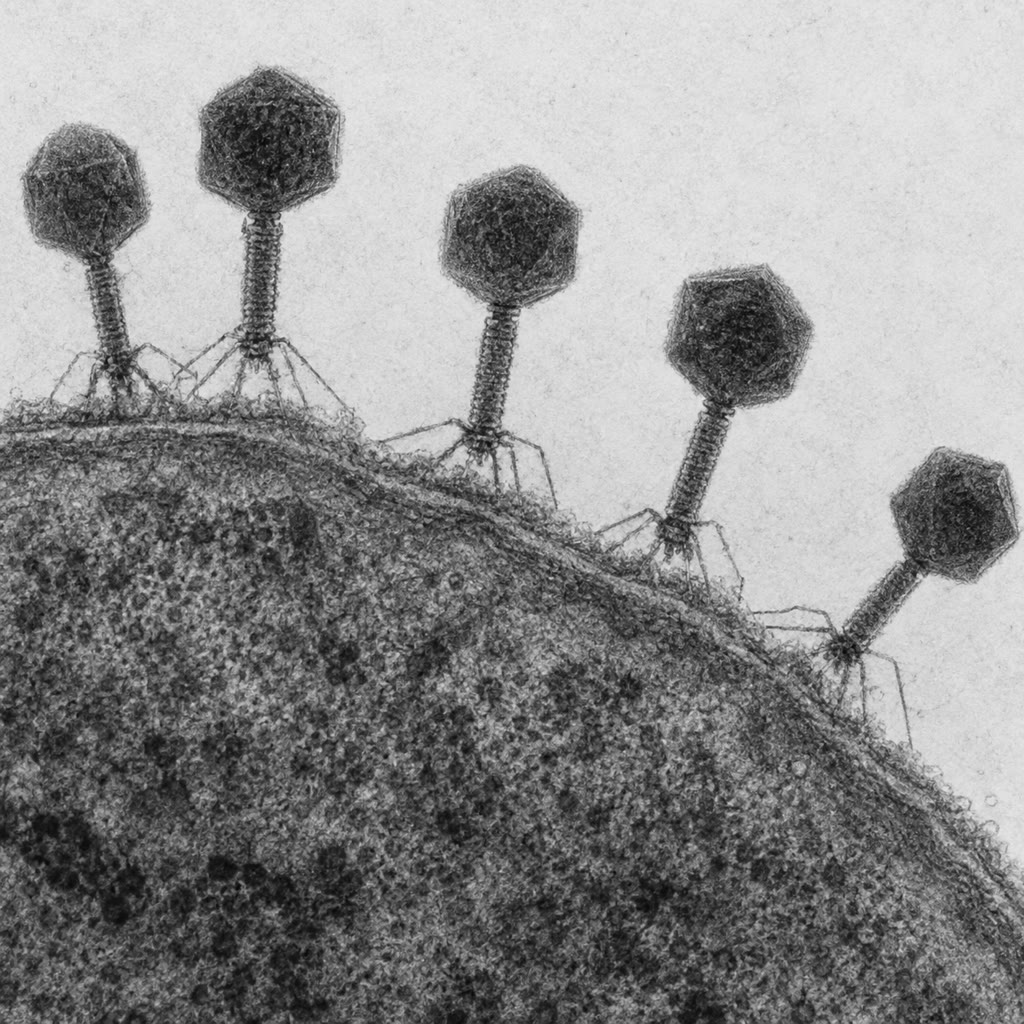
\includegraphics[width=0.36\linewidth]{images/book5/ai/b5-13-phage-tem.jpg}\hspace{0.04\linewidth}
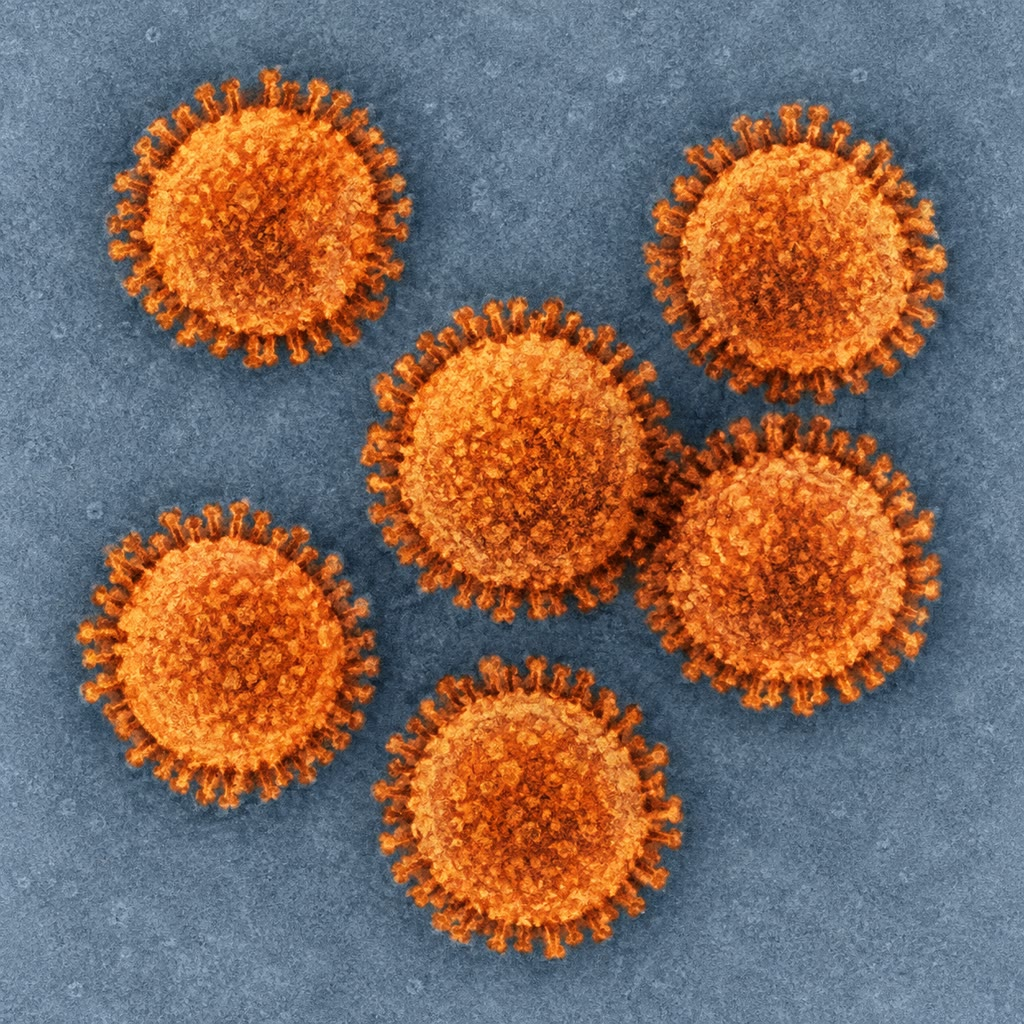
\includegraphics[width=0.36\linewidth]{images/book5/ai/b5-13-influenza-virions.jpg}

{\small Links: bacteriofagen die met hun staartvezels aan een bacterie
zijn gehecht, met elke kop een icosaëdrisch \omterm{def:b3:virology:virus}{capside} vol DNA. Rechts:
griepvirionen, met \omterm{def:b3:virology:virus}{envelop}, waarvan het oppervlak een franje van
hemagglutinine- en neuraminidasepieken draagt.}
\end{omfigure}

\section{Hoe een virus zich vermenigvuldigt}

\begin{definition}[De replicatiecyclus]\label{def:b3:virology:cycle}
\index{virale replicatiecyclus}\index{receptor!viraal}\index{lysogenie}\index{latentie}
Elk \omterm{def:b3:virology:virus}{virus} doorloopt dezelfde stadia. De \emph{hechting} aan een
bepaalde gastheerreceptor --- CD4 en een chemokinereceptor voor hiv,
ACE2 voor de SARS-coronavirussen, siaalzuur voor de griep, een
\omterm{def:b3:bacteriology:envelope}{lipopolysacharide} of een porine voor een faag --- die bepaalt welke
soorten en welke cellen het \omterm{def:b3:virology:virus}{virus} kan besmetten (zijn \emph{tropisme}).
De \emph{intrede}: fusie van de \omterm{def:b3:virology:virus}{envelop} met het plasmamembraan, of
endocytose gevolgd door fusie van binnenuit het zure \omterm{def:b3:membrane-traffic:endocytosis}{endosoom}, of, bij
een faag, injectie van het genoom door de wand. Het \emph{ontmantelen},
de \emph{expressie} van de virale genen langs de weg van de klasse, en
de \emph{replicatie} van het genoom, vaak in een fabriek die het \omterm{def:b3:virology:virus}{virus}
in het cytoplasma of de kern bouwt. De \emph{assemblage} van nieuwe
\omterm{def:b3:virology:virus}{capsiden} om nieuwe genomen heen, gedreven door het zelf samenstellen
van de symmetrische subeenheden, en de \emph{vrijlating}: door de cel
te doen barsten, of door door een membraan naar buiten te knoppen, wat
de \omterm{def:b3:virology:virus}{envelop} levert. Sommige virussen kunnen in plaats daarvan hun genoom
in dat van de gastheer invoegen en wachten: de \emph{lysogenie} van
faag $\lambda$, waarvan de repressor hem stil houdt tot de gastheer
beschadigd raakt; de \emph{latentie} van herpesvirussen in neuronen, een
leven lang, en van hiv als provirus in rustende T-cellen, waaruit geen
enkel middel dat op de replicatie werkt hem verwijdert.
\end{definition}

\begin{omfigure}
\begin{tikzpicture}[every node/.style={font=\scriptsize}, >=stealth]
  % cell
  \draw[very thick, omDef, fill=omDef!6] (0,0) ellipse (5.6 and 3.2);
  \draw[thick, omDef!70, fill=omDef!20] (1.8,0) ellipse (1.6 and 1.1); \node at (1.8,0.75) {kern};
  % virion outside
  \draw[thick, omProp, fill=omProp!30] (-7.2,1.6) circle (0.35); \foreach \a in {0,45,...,315} \draw[omProp, thick] (-7.2,1.6) ++(\a:0.35) -- ++(\a:0.15);
  \node[above] at (-7.2,2.1) {virion};
  \draw[->, thick] (-6.8,1.4) -- (-5.7,0.9); \node[below, align=center] at (-6.6,1.0) {1. hechten aan\\de receptor};
  % entry
  \draw[thick, omProp] (-5.4,0.7) arc[start angle=140, end angle=40, radius=0.5];
  \node[below, align=center] at (-3.9,-0.2) {2. fuseren of endocyteren;\\3. ontmantelen};
  % genome path
  \draw[omThm, very thick] (-3.4,0.2) .. controls (-2.6,0.6) .. (-1.8,0.4);
  \draw[->, thick] (-1.6,0.4) -- (-0.4,0.4);
  \node[above, align=center] at (-1.0,0.55) {4. genen tot expressie brengen,\\genoom repliceren};
  \draw[omThm, very thick] (-1.0,-0.5) -- (0.4,-0.5); \draw[omThm, very thick] (-1.0,-0.75) -- (0.4,-0.75); \draw[omThm, very thick] (-1.0,-1.0) -- (0.4,-1.0);
  % assembly
  \foreach \p in {(1.2,-1.6),(1.9,-1.9),(2.6,-1.5)} { \draw[thick, omProp, fill=omProp!30] \p circle (0.25); }
  \node[below, align=center] at (1.9,-2.2) {5. capsiden samenstellen\\om de genomen heen};
  % budding
  \draw[thick, omProp, fill=omProp!30] (4.9,-1.7) circle (0.32); \draw[->, thick] (5.3,-1.75) -- (6.4,-2.0);
  \draw[thick, omProp, fill=omProp!30] (7.0,-2.2) circle (0.35); \foreach \a in {0,45,...,315} \draw[omProp, thick] (7.0,-2.2) ++(\a:0.35) -- ++(\a:0.15);
  \node[below, align=center] at (6.4,-2.6) {6. door het membraan knoppen\\(envelop) of de cel doen barsten};
  % latency
  \draw[->, thick, dashed, omMeth!70!black] (-0.2,0.2) -- (0.9,0.2); \node[below, omMeth!70!black, align=center, font=\tiny] at (2.0,-0.05) {retrovirussen: integreren\\als provirus; latentie};
\end{tikzpicture}

{\small De replicatiecyclus van een \omterm{def:b3:virology:virus}{virus} met \omterm{def:b3:virology:virus}{envelop}: hechting aan een
receptor, intrede en ontmanteling, expressie en replicatie in de
machinerie van de gastheer, assemblage, en vrijlating door knopvorming
--- of, bij een retrovirus, integratie in het gastheergenoom en
stilte.}
\end{omfigure}

\begin{method}[Besmettelijke deeltjes tellen: de plaquetoets]\label{met:b3:virology:plaque}
\index{plaquetoets}\index{titer}
Om een virusvoorraad te meten: (1) verdun haar in stappen van tien;
(2) meng elke verdunning met een overmaat gastheercellen --- bacteriën
in zachte agar voor een faag, een laag gekweekte cellen voor een
diervirus; (3) laat groeien: elk besmettelijk deeltje besmet één cel,
het nageslacht besmet de buren, en na een dag of twee markeert een
helder gat, een \emph{plaque}, de plek; (4) tel de plaques op een plaat
met er \numrange{30}{300} en vermenigvuldig met de verdunning: de
\emph{titer} in plaquevormende eenheden (PVE) per milliliter. Omdat elke
plaque een kloon van één deeltje is, levert haar oppikken een zuiver
isolaat. De verhouding van fysieke deeltjes (geteld met de
elektronenmicroscoop of met PCR) tot plaquevormende eenheden ligt
meestal ver boven één --- tien tot duizend voor veel diervirussen ---
omdat de meeste deeltjes gebrekkig zijn of er niet in slagen te
besmetten.
\end{method}

\begin{omfigure}
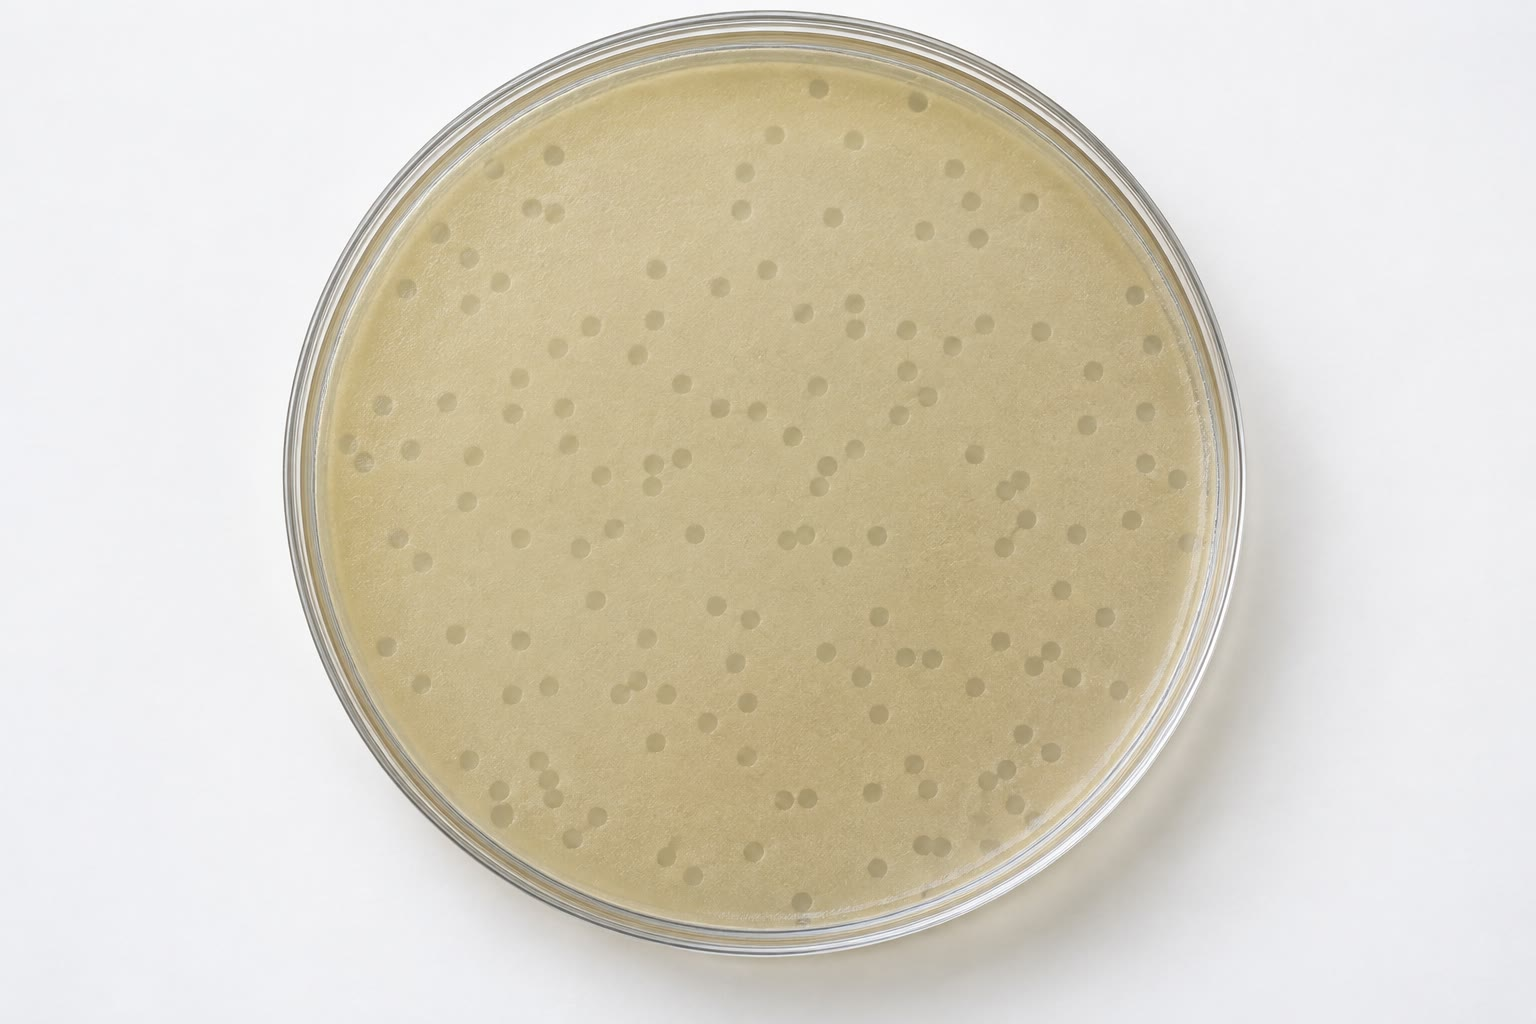
\includegraphics[width=0.46\linewidth]{images/book5/ai/b5-13-plaque-assay.jpg}\hspace{0.04\linewidth}
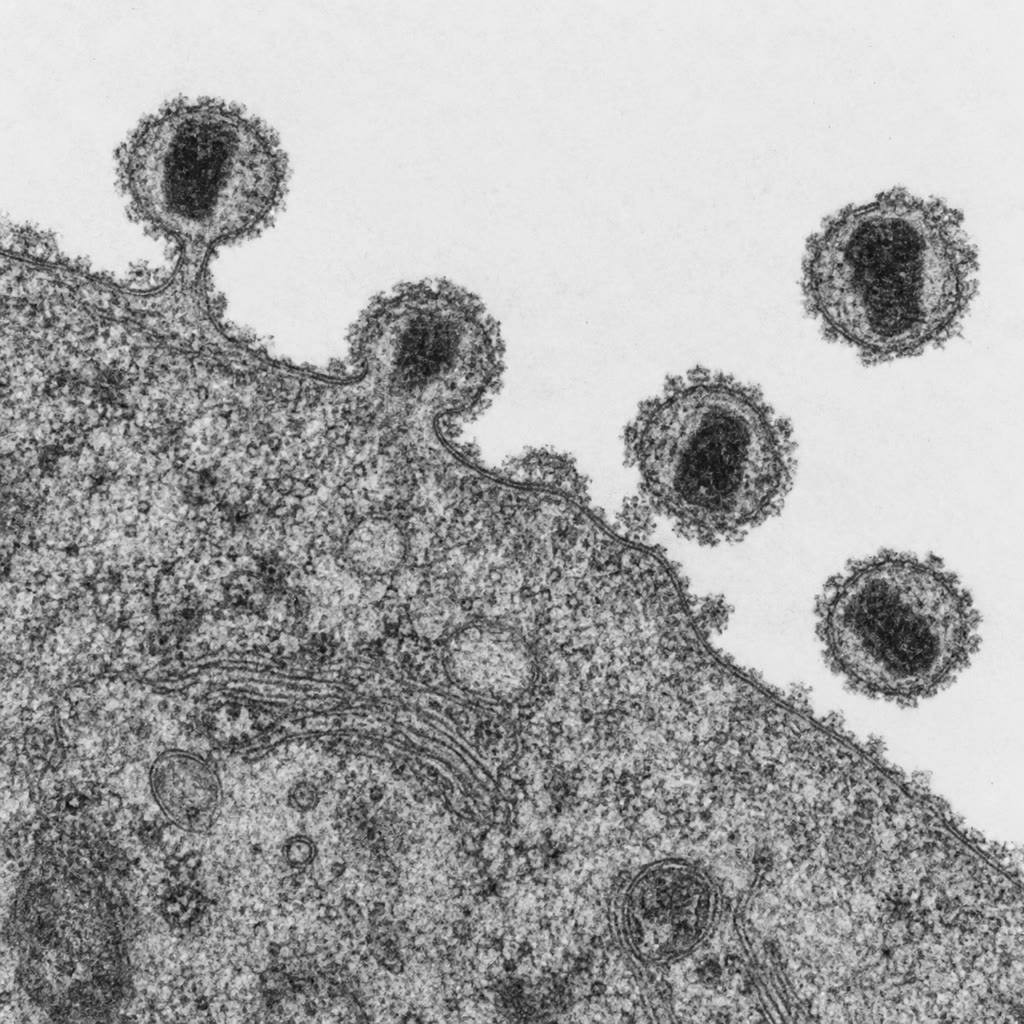
\includegraphics[width=0.36\linewidth]{images/book5/ai/b5-13-hiv-budding.jpg}

{\small Links: plaques in een bacterieveld, elk een heldere zone waar
het nageslacht van één faag de cellen eromheen heeft doen barsten.
Rechts: hiv-deeltjes die uit een T-lymfocyt knoppen en hun \omterm{def:b3:virology:virus}{envelop} aan
het membraan van de cel ontlenen.}
\end{omfigure}

\begin{theorem}[Infectiedynamiek binnen een gastheer]\label{thm:b3:virology:dynamics}
\index{basaal reproductiegetal!binnen de gastheer}\index{virale last}\index{virale dynamiek}
Zij $T$ de dichtheid van vatbare doelcellen, $I$ die van besmette cellen
en $V$ die van vrije \omterm{def:b3:virology:virus}{virionen}. \omterm{def:b3:virology:virus}{Virionen} besmetten doelcellen met
snelheid $\beta TV$, besmette cellen maken elk \omterm{def:b3:virology:virus}{virionen} met snelheid
$p$ en sterven met snelheid $\delta$, en vrije \omterm{def:b3:virology:virus}{virionen} worden
geklaard met snelheid $c$:
\[
\frac{\mathrm{d}I}{\mathrm{d}t} = \beta TV - \delta I, \qquad
\frac{\mathrm{d}V}{\mathrm{d}t} = pI - cV .
\]
Met $T$ constant gehouden groeit de infectie wanneer het \emph{basale
reproductiegetal} $R_{0} = \beta Tp/(c\delta)$ groter is dan $1$, en in
evenwicht geldt $V^{*} = p I^{*}/c$, waarbij de productie de klaring
opheft. Stopt een geneesmiddel op $t = 0$ alle nieuwe besmettingen
($\beta \to 0$), dan vervallen de \omterm{def:b3:virology:virus}{virionen} eerst met de klaringssnelheid
$c$ en daarna, zodra het vrije \omterm{def:b3:virology:virus}{virus} is gezakt tot het niveau dat de
overgebleven besmette cellen in stand houden, met de sterftesnelheid
$\delta$ van die cellen:
\[
V(t) \approx V_{0}\,\frac{c\,e^{-\delta t} - \delta\,e^{-ct}}{c - \delta}
\;\longrightarrow\; V_{0}\,\frac{c}{c-\delta}\,e^{-\delta t}
\quad (t \gg 1/c).
\]
De twee hellingen van de \omterm{thm:b3:virology:dynamics}{virale last} na de behandeling meten $c$ en
$\delta$, en $pI^{*} = cV^{*}$ geeft de dagelijkse productie van
\omterm{def:b3:virology:virus}{virionen} vóór de behandeling.
\end{theorem}
\begin{proof}
Een besmette cel leeft gemiddeld $1/\delta$ en maakt $p/\delta$
\omterm{def:b3:virology:virus}{virionen}; elk \omterm{def:b3:virology:virus}{virion} leeft $1/c$ en besmet in die tijd $\beta T/c$
cellen; het product is het aantal besmette cellen dat één besmette cel
voortbrengt, $R_{0}$. In evenwicht geeft $\mathrm{d}V/\mathrm{d}t = 0$
dat $V^{*} = pI^{*}/c$. Na de behandeling geldt
$\mathrm{d}I/\mathrm{d}t =
-\delta I$, dus $I = I_{0}e^{-\delta t}$, en is
$\mathrm{d}V/\mathrm{d}t =
pI_{0}e^{-\delta t} - cV$ een lineaire vergelijking waarvan de
oplossing met $V(0) = V_{0} = pI_{0}/c$ de gegeven uitdrukking is
(controle: bij $t = 0$ is zij gelijk aan $V_{0}$, en zij voldoet term
voor term aan de vergelijking). Voor $t
\gg 1/c$ is de term $e^{-ct}$ verdwenen en volgt $V$ de besmette cellen
met helling $-\delta$; voor $t \ll 1/\delta$ en $c \gg \delta$ is de
vroege helling $-c$.
\end{proof}

\begin{example}[Hiv vóór en na de vergelijkingen]\label{ex:b3:virology:hiv}
Tot 1995 werden de jaren van klinische \omterm{def:b3:virology:cycle}{latentie} bij een hiv-infectie ---
een stabiele \omterm{thm:b3:virology:dynamics}{virale last} van $10^{4}$--$10^{6}$ kopieën per milliliter
en een trage daling van de T-cellen --- gelezen als een sluimerend
\omterm{def:b3:virology:virus}{virus}. Ho, Perelson en collega's gaven patiënten een \omterm{def:b3:virology:drugs}{proteaseremmer} en
pasten de daling van de \omterm{thm:b3:virology:dynamics}{virale last} aan de stelling aan: de snelle fase
gaf $c \approx \qty{3}{d^{-1}}$ (een halveringstijd van een \omterm{def:b3:virology:virus}{virion} van
ongeveer zes uur), de trage fase $\delta \approx
\qty{0.5}{d^{-1}}$ (een besmette cel leeft ongeveer anderhalve dag).
Een stabiele last van $10^{5}$ per milliliter in \qty{15}{L}
lichaamsvocht, geklaard met $c$, vergt dus de productie van ongeveer
$10^{10}$ \omterm{def:b3:virology:virus}{virionen} per dag, elke dag, jarenlang: de ``latente'' periode
is een razende evenwichtstoestand van besmetting en dood, waarbij de
voorraad T-cellen dagelijks wordt vervangen tot zij het begeeft. De
mutatierekenkunde van de volgende paragraaf volgt daar meteen uit, en
daarmee de reden dat losse middelen faalden en drie niet.
\end{example}

\begin{omfigure}
\begin{tikzpicture}
\begin{axis}[
  width=0.7\linewidth, height=5.8cm,
  axis x line=bottom, axis y line=left,
  xmin=0, xmax=14, ymin=10, ymax=2e5, ymode=log,
  xlabel={dagen na het begin van de behandeling}, ylabel={virionen per mL},
  xlabel style={font=\small, at={(axis description cs:0.5,-0.12)}, anchor=north}, ylabel style={font=\small},
  tick label style={font=\small}, xtick={0,2,4,6,8,10,12,14},
  clip=false,
]
\addplot[very thick, omDef, domain=0:14, samples=100] {1e5*(3*exp(-0.5*x) - 0.5*exp(-3*x))/2.5};
\addplot[dashed, omThm, domain=0:1.6, samples=2] {1e5*exp(-3*x)};
\addplot[dashed, omMeth!70!black, domain=1.5:14, samples=2] {1e5*1.2*exp(-0.5*x)};
\node[font=\scriptsize, omThm, anchor=west] at (axis cs:1.8,600) {vrije virionen geklaard: helling $-c$, halveringstijd \qty{6}{h}};
\node[font=\scriptsize, omMeth!70!black, anchor=south west] at (axis cs:5.5,1.5e4) {besmette cellen sterven: helling $-\delta$, halveringstijd \qty{1.4}{d}};
\end{axis}
\end{tikzpicture}

{\small De \omterm{thm:b3:virology:dynamics}{virale last} nadat een middel nieuwe besmettingen heeft
gestopt, volgens de stelling met $c = \qty{3}{d^{-1}}$ en
$\delta = \qty{0.5}{d^{-1}}$: een snelle daling terwijl vrije \omterm{def:b3:virology:virus}{virionen}
worden geklaard, daarna een tragere daling op het tempo van het sterven
van de reeds besmette cellen.}
\end{omfigure}

\section{Hoe virussen evolueren}

\begin{definition}[Mutatie, quasisoort, drift en shift]\label{def:b3:virology:evolution}
\index{quasisoort}\index{antigene drift}\index{antigene shift}\index{herschikking}
RNA-afhankelijke polymerasen en reverse transcriptasen lezen hun werk
niet na, en RNA-virussen muteren met $10^{-4}$ tot $10^{-6}$ per
nucleotide per replicatie --- duizend tot een miljoen keer de snelheid
van hun gastheren --- zodat een populatie van een \omterm{def:b3:virology:virus}{RNA-virus} een wolk
verwante genomen is, een \emph{quasisoort}, waarin elke afzonderlijke
puntmutant altijd aanwezig is als de populatie groot is. De selectie
door antilichamen drijft de \emph{antigene drift}: de
oppervlakte-eiwitten van het griepvirus stapelen jaar na jaar
substituties op, en de afweer van vorig jaar beschermt elk seizoen
minder. De \emph{antigene shift} is een sprong: een genoom in segmenten
(het griepvirus heeft acht RNA-segmenten) kan worden
\emph{herschikt} wanneer twee stammen één cel besmetten, en een segment
dat codeert voor een hemagglutinine van een vogel- of varkensvirus,
waartegen geen mens afweer heeft, brengt een pandemie voort --- 1918,
1957, 1968, 2009. De recombinatie binnen een genoom doet hetzelfde voor
virussen zonder segmenten, en de coronavirussen recombineren vrijelijk.
De meeste nieuwe menselijke virussen zijn \emph{zoönosen} die uit een
dierlijk reservoir overspringen --- vleermuizen voor de coronavirussen,
ebola en hondsdolheid; vogels en varkens voor de griep; primaten voor
hiv --- en het overspringen is meestal een kwestie van enkele mutaties
in een receptorbindend eiwit.
\end{definition}

\begin{proposition}[De foutendrempel]\label{prop:b3:virology:error-threshold}
\index{foutendrempel}\index{nalezen!viraal}
Een genoom van $L$ nucleotiden dat met foutenpercentage $u$ per
nucleotide wordt gekopieerd, wordt zonder enige fout gekopieerd met
kans $(1-u)^{L} \approx e^{-uL}$. Wil de fitste sequentie in de
populatie standhouden tegen de vloed van haar mutanten, dan moet het
deel foutloze kopieën ongeveer boven het omgekeerde van haar selectieve
voordeel $\sigma$ liggen: $e^{-uL} \gtrsim
1/\sigma$, dat wil zeggen $uL \lesssim \ln\sigma$, een getal van de
orde één. Het product van mutatiesnelheid en genoomlengte is dus
begrensd: een \omterm{def:b3:virology:virus}{RNA-virus} met $u = 10^{-4}$ kan geen genoom hebben dat
veel langer is dan $10^{4}$ nucleotiden, en dat is ongeveer wat
RNA-virussen hebben; de coronavirussen, met \qty{30}{kb} de langste
bekende RNA-genomen, halen dat alleen door voor een nalezend
exonuclease te coderen dat $u$ tienvoudig verlaagt. De drempel is ook
een wapen: middelen die het foutenpercentage van het polymerase
verhogen (ribavirine, molnupiravir) duwen een \omterm{def:b3:virology:virus}{virus} eroverheen tot in
de \emph{foutencatastrofe}, en de \omterm{def:b3:virology:evolution}{quasisoort} stort in.
\end{proposition}
\begin{proof}
Onafhankelijke fouten op elk van $L$ plaatsen geven de kans op
foutloosheid $(1-u)^{L}$, en $\ln(1-u) \approx -u$ voor kleine $u$. De
populatiebalans is het gebruikelijke argument van de \omterm{def:b3:virology:evolution}{quasisoort} (Eigen,
1971): de meestersequentie wordt ten opzichte van de gemiddelde mutant
aangevuld met snelheid $\sigma e^{-uL}$ en gaat verder aan mutatie
verloren; zij blijft alleen bestaan als het eerste groter is dan $1$,
waaruit de grens volgt.
\end{proof}

\begin{omfigure}
\begin{tikzpicture}[every node/.style={font=\scriptsize}, >=stealth]
  % drift
  \begin{scope}
    \foreach \i in {0,1,2,3} { \draw[thick, omProp, fill=omProp!30] (\i*1.3,0) circle (0.35); \foreach \a in {0,60,...,300} \draw[omProp, thick] (\i*1.3,0) ++(\a:0.35) -- ++(\a:0.14); }
    \foreach \i/\n in {1/1,2/2,3/3} { \foreach \k in {1,...,\n} \fill[omThm] (\i*1.3,0) ++({60*\k+20}:0.5) circle (0.06); }
    \foreach \i in {0,1,2} \draw[->, thick] (\i*1.3+0.5,0) -- (\i*1.3+0.8,0);
    \node[below, align=center] at (1.95,-0.6) {antigene drift: puntmutaties hopen zich\\seizoen na seizoen op\\in de oppervlakte-eiwitten};
  \end{scope}
  % shift
  \begin{scope}[xshift=7.0cm]
    \draw[thick, omProp, fill=omProp!30] (0,0.5) circle (0.4); \foreach \y in {-0.2,-0.1,0,0.1,0.2} \draw[omProp!80!black] (-0.25,0.5+\y) -- (0.25,0.5+\y);
    \draw[thick, omMeth!70!black, fill=omMeth!30] (0,-0.7) circle (0.4); \foreach \y in {-0.2,-0.1,0,0.1,0.2} \draw[omMeth!70!black] (-0.25,-0.7+\y) -- (0.25,-0.7+\y);
    \node[left, align=right] at (-0.5,0.5) {menselijke stam,\\8 segmenten}; \node[left, align=right] at (-0.5,-0.7) {vogelstam,\\8 segmenten};
    \draw[->, thick] (0.5,0.4) -- (1.5,0.0); \draw[->, thick] (0.5,-0.6) -- (1.5,-0.2);
    \draw[thick, omDef, fill=omDef!10] (2.4,-0.1) ellipse (0.9 and 0.7); \node[below] at (2.4,-0.85) {één cel (een varken)};
    \draw[->, thick] (3.4,-0.1) -- (4.3,-0.1);
    \draw[thick, omProp, fill=omProp!30] (4.9,-0.1) circle (0.4); \foreach \y in {-0.2,-0.1,0.1,0.2} \draw[omProp!80!black] (4.65,-0.1+\y) -- (5.15,-0.1+\y); \draw[omMeth!70!black, very thick] (4.65,-0.1) -- (5.15,-0.1);
    \node[right, align=left] at (5.4,-0.1) {herschikking: vogel-\\hemagglutinine in\\een menselijk virus};
    \node[below, align=center] at (2.4,-1.5) {antigene shift: hele segmenten\\uitgewisseld; niemand heeft\\afweer --- een pandemie};
  \end{scope}
\end{tikzpicture}

{\small Twee manieren waarop een griepvirus aan de afweer ontsnapt.
Drift: mutaties in de pieken hopen zich geleidelijk op. Shift: twee
stammen in één cel wisselen hele genoomsegmenten uit, en er verschijnt
in één keer een piekeiwit dat nieuw is voor de mens.}
\end{omfigure}

\begin{example}[Waarom hiv drie middelen nodig had]\label{ex:b3:virology:three-drugs}
Het reverse transcriptase van hiv vergist zich ongeveer eens per
$10^{5}$ nucleotiden, zodat elk gekopieerd genoom van \qty{9700}{nt}
ongeveer $0.1$ mutaties draagt, en $10^{10}$ nieuwe genomen per dag
samen $10^{9}$ mutaties dragen: elk van de
$3\times 9700 \approx \num{30000}$ mogelijke enkele puntmutaties
ontstaat elke dag vele keren, nog voordat er een middel is gegeven. Een
middel dat één enkele mutatie verslaat --- zoals één mutatie de meeste
remmers van het reverse transcriptase en van het protease verslaat ---
is daarom binnen weken verslagen, en dat is wat AZT in 1987 overkwam.
Twee onafhankelijke mutaties ontstaan samen met $10^{-10}$ per genoom,
ongeveer eens per dag; drie met $10^{-15}$, eens per duizend dagen ---
en een patiënt op drie middelen wiens last duizendvoudig is gedaald
maakt $10^{7}$ genomen per dag, zodat de drievoudige mutant nooit
verschijnt. Dat, en het bewijs uit de stelling dat het \omterm{def:b3:virology:virus}{virus} op volle
snelheid repliceerde, maakten de \omterm{thm:b3:cancer-biology:goldie-coldman}{combinatietherapie} vanaf 1996 tot de
behandeling die van aids een chronische aandoening maakte.
\end{example}

\section{Gastheren, afweer en geneesmiddelen}

\begin{proposition}[Ziekmakend vermogen en afweer]\label{prop:b3:virology:pathogenesis}
\index{cytopathisch effect}\index{interferon}\index{restrictie!faag}
Een \omterm{def:b3:virology:virus}{virus} richt schade aan door cellen te doen barsten (polio vernielt
motorische neuronen, hiv doodt T-cellen), door cellen giftige producten
te laten maken, door ze te transformeren
(\cref{ch:b3:cancer-biology}), en vaak vooral via de eigen reactie van
de gastheer: de koorts, de weefselschade en, in het ergste geval, de
cytokinestorm van de afweerreactie op de griep of de
SARS-coronavirussen. De gastheer antwoordt met aangeboren afweer die de
handtekeningen van virale replicatie herkent --- dubbelstrengs RNA, RNA
zonder kap, DNA in het cytosol --- en met \emph{interferon} reageert,
dat elke buurcel in een antivirale toestand brengt
(\cref{ch:b3:innate-immunity}); met natuurlijke doodcellen die cellen
vernietigen die hun MHC hebben verborgen; met antilichamen die \omterm{def:b3:virology:virus}{virionen}
onschadelijk maken en cytotoxische T-cellen die besmette cellen doden
voordat zij nageslacht vrijlaten
(\cref{ch:b3:adaptive-immunity}); en, bij bacteriën, met
\omterm{def:b3:genetic-engineering:tools}{restrictie-enzymen} die vreemd DNA knippen en het CRISPR-geheugen van
\cref{ch:b3:genetic-engineering}. De virussen antwoorden terug: vrijwel
elk groot \omterm{def:b3:virology:virus}{virus} codeert eiwitten die het interferon blokkeren, het MHC
verbergen, cytokinen nabootsen of de \omterm{def:b3:cell-cycle-apoptosis:apoptosis}{apoptose} remmen, en de wapenwedloop
staat in beide genomen geschreven.
\end{proposition}

\begin{definition}[Antivirale middelen en vaccins]\label{def:b3:virology:drugs}
\index{antiviraal middel}\index{nucleoside-analoog}\index{proteaseremmer}\index{vaccin}\index{mRNA-vaccin}
Antivirale middelen vallen de virale enzymen aan of de stappen die een
gastheercel niet uitvoert. \emph{Nucleoside-analogen} zijn
ketenafbrekers: aciclovir wordt alleen door het thymidinekinase van het
herpesvirus gefosforyleerd en blokkeert daarna het virale
DNA-polymerase, zodat het alleen in besmette cellen werkt; AZT,
tenofovir en lamivudine stoppen het reverse transcriptase; remdesivir en
molnupiravir werken op het polymerase van het coronavirus, het tweede
door mutagenese. \emph{Proteaseremmers} blokkeren het knippen van
virale polyproteïnen (hiv, hepatitis C, het nirmatrelvir tegen
SARS-CoV-2). Integraseremmers verhinderen dat het provirus van hiv
ontstaat; neuraminidaseremmers beletten dat griepvirionen loslaten van
de cel waaruit zij knoppen; intrederemmers blokkeren een receptor. Het
hepatitis-C-virus wordt nu in twaalf weken genezen met combinaties van
rechtstreeks werkende middelen, de eerste chronische virusinfectie die
ooit met chemotherapie is genezen. \emph{Vaccins} bieden de antigenen
van het \omterm{def:b3:virology:virus}{virus} zonder zijn ziekte: een levend verzwakt \omterm{def:b3:virology:virus}{virus} (mazelen,
polio via de mond, gele koorts), een geïnactiveerd \omterm{def:b3:virology:virus}{virus} (polio per
injectie, griep), een subeenheid (het oppervlakteantigeen van hepatitis
B gemaakt in gist, het capside-eiwit van het papillomavirus), een
onschadelijke virale \omterm{def:b3:genetic-engineering:tools}{vector} met een gen van het doelwit, of, sinds
2020, \emph{boodschapper-RNA} dat voor het antigeen codeert, geleverd
in lipidenanodeeltjes, dat de eigen cellen van de ontvanger vertalen.
De immunologie van waarom zij werken, en van hoeveel mensen er moeten
worden ingeënt om de rest te beschermen, is de stof van
\cref{ch:b3:adaptive-immunity}.
\end{definition}

\begin{remark}[Virussen in de huishouding van het leven]\label{rem:b3:virology:economy}
De virussen die de mens schaden zijn een afrondingsfout in de
viruspopulatie van de wereld, waarvan het meeste bacteriën en archaea
besmet. Fagen doden dagelijks een vijfde tot een derde van de bacteriën
in de oceaan en geven hun inhoud terug aan de opgeloste voorraad --- de
\emph{virale nevenweg} van de koolstofkringloop uit het boek van
jaar~2. Zij verplaatsen genen tussen bacteriën
(\cref{ch:b3:bacteriology}), en hun toxinen zijn de toxinen van
difterie, cholera en de ergste \emph{E.~coli}. Acht procent van het
menselijk genoom bestaat uit de resten van oude retrovirussen
(\cref{ch:b3:genomics}), en een van hun envelopgenen versmelt nu de
cellen van de placenta. Virussen zijn het grootste reservoir van
genetische nieuwigheid op de planeet, en de grens van wat als levend
telt loopt dwars door hen heen.
\end{remark}

\section{Opgaven}

\begin{exercise}[$\star$]\label{exo:b3:virology:1}
Plaats polio, griep, hiv, herpes simplex, hepatitis B en rotavirus in
hun klassen van Baltimore en zeg welk enzym elk moet meebrengen of
maken dat de cel mist.
\end{exercise}

\begin{exercise}[$\star$]\label{exo:b3:virology:2}
Wat toonde het experiment van Hershey en Chase aan, en wat zou er zijn
gevonden als het eiwit de instructies had gedragen?
\end{exercise}

\begin{exercise}[$\star$]\label{exo:b3:virology:3}
Een faagvoorraad die $10^{-7}$ is verdund geeft $84$ plaques uit
\qty{0.1}{mL}. Wat is de titer? Waarom kan de elektronenmicroscoop tien
keer meer deeltjes tellen?
\end{exercise}

\begin{exercise}[$\star$]\label{exo:b3:virology:4}
Noem de zes stadia van een replicatiecyclus en bij elk één \omterm{def:b3:virology:drugs}{antiviraal
middel} of één afweermiddel van de gastheer dat erop ingrijpt.
\end{exercise}

\begin{exercise}[$\star\star$]\label{exo:b3:virology:5}
Bereken met \cref{prop:b3:virology:economy} het nucleïnezuur dat nodig
is om het \omterm{def:b3:virology:virus}{capside} te coderen van een \omterm{def:b3:virology:virus}{virus} dat uit $180$ kopieën van
een eiwit van \qty{30}{kDa} bestaat, en vergelijk met het genoom van
\qty{4.5}{kb} dat zo'n \omterm{def:b3:virology:virus}{virus} zou kunnen hebben. Welk deel van het
genoom is het capsidegen?
\end{exercise}

\begin{exercise}[$\star\star$]\label{exo:b3:virology:6}
Bereken met $c = \qty{3}{d^{-1}}$, $\delta = \qty{0.5}{d^{-1}}$ en $V_{0} =
10^{5}$ per mL de waarde van $V$ uit de stelling bij $t = 0.5$, $2$ en
$10$ dagen. Hoe lang duurt het voordat de last onder $50$ per mL zakt,
de aantoonbaarheidsgrens?
\end{exercise}

\begin{exercise}[$\star\star$]\label{exo:b3:virology:7}
Een \omterm{def:b3:virology:virus}{RNA-virus} heeft $u = 3\times 10^{-5}$ en $L = \qty{12}{kb}$. Welk
deel van zijn nakomelingengenomen draagt geen enkele mutatie? Wat
gebeurt er met dat deel als een mutageen middel $u$ verdrievoudigt? Leg
uit waarom de coronavirussen een nalezend enzym nodig hadden.
\end{exercise}

\begin{exercise}[$\star\star$]\label{exo:b3:virology:8}
Leg de \omterm{def:b3:virology:evolution}{antigene drift} en shift bij het griepvirus uit, en waarom een
pandemische stam tot nu toe altijd een nieuw hemagglutinine droeg.
\end{exercise}

\begin{exercise}[$\star\star$]\label{exo:b3:virology:9}
Aciclovir is een guanosineanaloog dat moet worden gefosforyleerd om te
werken. Leg uit waarom het cellen met herpes schaadt en andere niet, en
voorspel de resistentiemutaties.
\end{exercise}

\begin{exercise}[$\star\star\star$]\label{exo:b3:virology:10}
Leid $R_{0} = \beta Tp/(c\delta)$ af uit de twee vergelijkingen van de
stelling door de voorwaarde te zoeken waaronder een kleine infectie
($I$ en $V$ bij nul, $T$ constant) groeit, en geef de betekenis van
elke factor.
\end{exercise}

\begin{exercise}[$\star\star\star$]\label{exo:b3:virology:11}
Een patiënt op werkzame therapie herbergt nog altijd $10^{6}$ latent
besmette rustende T-cellen waarvan het provirus zwijgt, met een
halveringstijd van $44$ maanden. Hoe lang zou de therapie moeten
voortduren voordat het reservoir onder één cel zakt? Waarom maakt dit
hiv ongeneeslijk met middelen die de replicatie blokkeren, en wat zou
een genezing vergen?
\end{exercise}

\begin{exercise}[$\star\star\star$]\label{exo:b3:virology:12}
Leg het argument van \cref{ex:b3:virology:three-drugs} uit met eigen
getallen voor een \omterm{def:b3:virology:virus}{virus} van \qty{30}{kb} met $u = 10^{-6}$ dat $10^{9}$
genomen per dag maakt. Hoeveel middelen zouden er moeten worden
gecombineerd, en waarom tellen middelen tegen twee plaatsen van
hetzelfde enzym mogelijk niet als twee?
\end{exercise}

\section{Vraagstuk: een virus in een patiënt}

\begin{problem}[{Weekendvraagstuk --- een hiv-infectie virion voor
virion geteld, haar dynamiek aangepast aan een behandelcurve, haar
mutaties tegen de middelen afgezet, en haar reservoir in de tijd gezet,
met als besluit de dagelijkse productie van virionen, de dag waarop de
last onaantoonbaar wordt en de kans dat er een drievoudige mutant
bestaat}]
\label{pb:b3:virology:1}
Gegevens: \omterm{thm:b3:virology:dynamics}{virale last} $V^{*} = 2\times 10^{5}$ per mL in \qty{15}{L}
lichaamsvocht; $c = \qty{3}{d^{-1}}$, $\delta = \qty{0.5}{d^{-1}}$; elke
besmette cel maakt $p = 500$ \omterm{def:b3:virology:virus}{virionen} per dag; genoom \qty{9700}{nt},
$u = 10^{-5}$ per nucleotide per replicatie; enkele mutaties geven
resistentie tegen elk van drie middelen; op drievoudige therapie daalt
de productie tot $10^{7}$ genomen per dag; latent reservoir $10^{6}$
cellen, halveringstijd $44$ maanden; een \omterm{def:b3:virology:virus}{virion} is een bol van
\qty{120}{nm} met twee RNA-strengen van \qty{9700}{nt} en ongeveer
\num{2000} eiwitmoleculen van \qty{25}{kDa}.

\medskip
\noindent\textbf{Deel I --- Tellen.}
\begin{enumerate}
  \item Hoeveel \omterm{def:b3:virology:virus}{virionen} zitten er in evenwicht in het lichaam?
  \item Hoeveel worden er per dag geklaard, en dus per dag gemaakt?
  \item Hoeveel besmette cellen maken ze, en hoeveel sterven er per
        dag?
  \item Wat is de massa van één \omterm{def:b3:virology:virus}{virion} (RNA à \qty{330}{Da} per
        nucleotide plus eiwit), en de totale massa van de \omterm{def:b3:virology:virus}{virionen} in
        het lichaam? Vergelijk met een zandkorrel (\qty{1}{mg}).
  \item Het lichaam heeft $10^{12}$ CD4-T-cellen en vervangt de besmette
        cellen. Welk deel van de voorraad is op enig moment besmet, en
        hoe doodt zo'n klein deel de voorraad in tien jaar?
  \item Als elke besmette cel door \omterm{def:b3:cell-cycle-apoptosis:apoptosis}{apoptose} sterft en binnen een uur
        wordt verzwolgen (\cref{ch:b3:cell-cycle-apoptosis}), hoeveel
        worden er op enig moment opgeruimd?
\end{enumerate}

\medskip
\noindent\textbf{Deel II --- Behandeling.}
\begin{enumerate}[resume]
  \item De therapie stopt op $t = 0$ alle nieuwe besmettingen. Bereken
        $V$ met de stelling bij $t =
        1$, $3$, $7$ en $14$ dagen.
  \item Op welke dag zakt de last onder de aantoonbaarheidsgrens van
        $50$ per mL?
  \item Hoe zou een arts uit de twee hellingen $c$ en $\delta$ schatten
        uit metingen op de dagen $0$--$1$ en $3$--$10$?
  \item Na de twee fasen vlakt de last af op enkele kopieën per mL en
        blijft daar jarenlang. Welk compartiment van het model ontbreekt
        er, en wat is de vervalsnelheid ervan?
  \item Bereken de halveringstijd van een vrij \omterm{def:b3:virology:virus}{virion} en van een besmette
        cel.
  \item Leg uit waarom het plateau vóór de behandeling ten onrechte als
        \omterm{def:b3:virology:cycle}{latentie} werd gelezen, en wat de vergelijkingen in plaats
        daarvan lieten zien.
\end{enumerate}

\medskip
\noindent\textbf{Deel III --- Mutatie.}
\begin{enumerate}[resume]
  \item Het aantal mutaties per genoom per replicatie, en het aantal
        mutaties dat bij de onbehandelde patiënt per dag ontstaat.
  \item Hoeveel verschillende enkele puntmutaties zijn er in het genoom
        mogelijk? Hoe vaak per dag ontstaat elk daarvan?
  \item De snelheid per genoom van een bepaalde dubbele mutant en van
        een bepaalde drievoudige mutant; hoeveel van elk ontstaan er per
        dag zonder behandeling?
  \item Hoeveel drievoudige mutanten zijn er op drievoudige therapie, met
        $10^{7}$ genomen per dag, per jaar te verwachten?
  \item De patiënt slaat doses over, zodat het niveau van één middel een
        week lang tot nul zakt terwijl de andere twee standhouden.
        Welke mutanten kunnen nu worden geselecteerd, en hoeveel van de
        betreffende dubbele mutanten zijn er in die week te verwachten
        bij $10^{7}$ genomen per dag?
  \item Waarom geeft resistentie tegen het ene \omterm{def:b3:virology:drugs}{nucleoside-analoog} vaak
        ook resistentie tegen het andere, en hoe verandert dat de
        telling van ``onafhankelijke'' middelen?
\end{enumerate}

\medskip
\noindent\textbf{Deel IV --- Het reservoir en de genezing.}
\begin{enumerate}[resume]
  \item Hoe lang duurt het bij een halveringstijd van $44$ maanden
        voordat de $10^{6}$ latente cellen tot één zijn gedaald? En tot
        $10^{4}$?
  \item Wordt de therapie gestopt, dan volstaat één latente cel die
        weer actief wordt om de infectie te hervatten. Hoe lang na het
        stoppen keert de last terug op $10^{5}$ per mL, als zij vanuit
        één \omterm{def:b3:virology:virus}{virion} met $R_{0} = 8$ per generatie van $2$ dagen groeit?
  \item Stel twee strategieën voor een genezing voor die uit het model
        volgen, en geef bij elk de hindernis.
  \item Het $R_{0}$ van de stelling geldt binnen één gastheer. Een
        $R_{0}$ voor hiv tussen mensen is ongeveer $3$--$5$. Welk deel
        van de overdrachten moet worden voorkomen om de epidemie te
        beëindigen ($1 - 1/R_{0}$)?
  \item Een behandeling verlaagt de besmettelijkheid van een patiënt
        vrijwel tot nul. Leg uit hoe ``behandeling als preventie'' uit
        de stelling binnen de gastheer volgt.
  \item Een \omterm{def:b3:virology:drugs}{vaccin} met werkzaamheid $E$ (het deel van de gevaccineerde
        mensen dat is beschermd) dat aan een deel $f$ van de bevolking
        wordt gegeven beschermt $Ef$ daarvan. Welke dekking $f$ is er
        nodig om de drempel van de vorige vraag te halen bij $E = 0.7$?
        En bij $E = 0.9$? Wat betekent het eerste antwoord?
  \item Vat samen: het aantal \omterm{def:b3:virology:virus}{virionen} dat per dag wordt gemaakt
        (vraag~2), de dag waarop de last onaantoonbaar wordt (vraag~8),
        en het verwachte aantal drievoudige mutanten per jaar onder
        therapie (vraag~16).
\end{enumerate}
\end{problem}
